% Szglab4
% ===========================================================================
%
\chapter{Szkeleton tervezése}

\thispagestyle{fancy}

\section{A szkeleton modell valóságos use-case-ei}

\subsection{Use-case diagram}
\comment{Kisebb problémám akadt a diagrammal, szerettem volna minél szebben megcsinálni (UGRÁS-ba extend nyíl: checkpointugrás, ragacs/olajba ugrás, meghalás) csak most melyik aktorhoz melyik tartozik kicsit belezavarodtam /Attó}

\begin{figure}[h]
\begin{center}
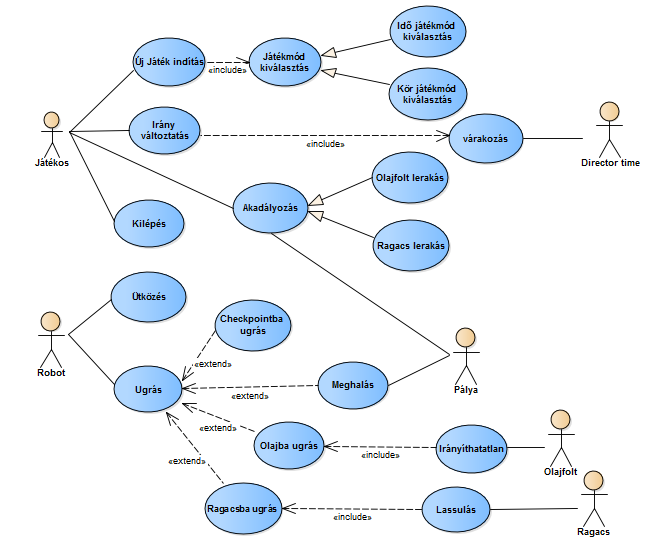
\includegraphics[width=17cm]{skeleton_use_case3.PNG}
\caption{x}
\label{fig:SzkeletonUseCase}
\end{center}
\end{figure}
\newpage

\subsection{Use-case leírások}
\comment{Szerintem bele lehetne venni a use-case-ekbe még a "robottal való ütközés"-t és a "checkpoint-ba ugrás"-t is. //Winnie}
\comment{Egyetértek, javítva, megoldva! ;) //Attó}

\usecase{Új játék indítása}{A játékos elindítja a játékot.}{Játékos}{A grafikus felületen (menüben) a felhasználó rákattinthat az „Új Játék indítása” menüpontra.}
\usecase{Irányváltoztatás}{A robot irányának beállítása.}{Játékos}{A robot ugrása előtt lehetőség van beállítani az irányát 3 másodpercig.}
\usecase{Játékmód kiválasztás}{Választás a játékmódok közül}{Játékos}{A játékos tud választani két játékmód közül, hogy milyen játékmódban szeretne játszani.}
\usecase{Checkpointba ugrás}{A robot beleugrik egy checkpointba.}{Robot}{A robot körmegtételének ellenőrzése miatt a robotnak checkpointokba kell beleugrálnia.}
\usecase{Ütközés}{Robotok ütköznek}{Robot}{Két robot összeütközése után lepattannak egymásról.}
\usecase{Idő játékmód kiválasztása}{A játékos kiválasztja az idő játékmódot.}{Játékos}{A grafikus felületen (menüben) a felhasználó olyan játékmódban indítja el a játékot amiben egy számláló fut visszafelé, és ha lejár, vége a játéknak.}
\newpage
\usecase{Kör játékmód kiválasztása}{A játékos kiválasztja a kör játékmódot.}{Játékos}{A grafikus felületen (menüben) a felhasználó olyan játékmódban indítja el a játékot, melyben el kell érni egy megadott körszámot, és ezután ér véget a játék.}
\usecase{Ugrás}{A robot ugrik a megadott irányba.}{Robot}{A játékos a megadott billentyűkkel beállítja az ugrás irányát, majd a robot ugrik.}
\usecase{Várakozás}{Egy számláló 3 másodpercig visszaszámol.}{Director time}{A körökre osztás miatt a robot csak három másodpercenként ugrik.}
\usecase{Meghalás}{A robot meghal.}{Pálya}{Az ugrás után, ha a robot nem tartózkodik a pályán, akkor meghal.}
\usecase{Akadályozás}{A pályára akadályok kerülnek.}{Játékos, Pálya}{A játékos utasíthatja a robotot, hogy rakjon le akadályt a pályára, illetve a pályára is kerülnek akadályok a játék elején.}
\usecase{Ragacs lerakás}{A pályára ragacs kerül.}{Játékos}{A robot ragacsot rak le a pályára a játékos utasítására.}
\usecase{Olajfolt lerakás}{A pályára olajfolt kerül.}{Játékos}{A robot olajfoltot rak le a pályára a játékos utasítására.}
\newpage
\usecase{Olajba ugrás}{A játékos olajfoltba ugrik.}{Robot}{A robot az ugrás után egy olajfoltra érkezik a pályán.}
\usecase{Irányíthatatlan}{A robot irányíthatatlan lesz.}{Olajfolt}{A játékos nem fogja tudni megváltoztatni a következő körben a robot ugrásának irányát, az „csúszni” fog tovább.}
\usecase{Ragacsba ugrás}{A játékos ragacsba ugrik.}{Robot}{A robot az ugrás után egy ragacsba érkezik a pályán.}
\usecase{Lassulás}{A robot sebessége a felére csökken.}{Ragacs}{Ha a robot ragacsba ugrik a pályán, akkor sebessége a felére csökken, a következő körben nem tud akkorát ugrani.}
\usecase{Kilépés}{A játékos kilép a játékból.}{Játékos}{A felhasználó visszalép a menübe, vagy teljesen leállítja a játék működését.}


\section{A szkeleton kezelői felületének terve, dialógusok}
\comment{A szkeleton által elfogadott bemenetek , valamint a szöveges konzolon megjelenő kimenetek. A kiemenet formátuma olyan kell legyen, ami alapján a működés összevethető a korábbi szekvencia-diagramokkal.}

\section{Szekvencia diagramok a belső működésre}

\pagebreak
\subsection{Robot::CheckpointSearch}
\begin{figure}[h]
\begin{center}
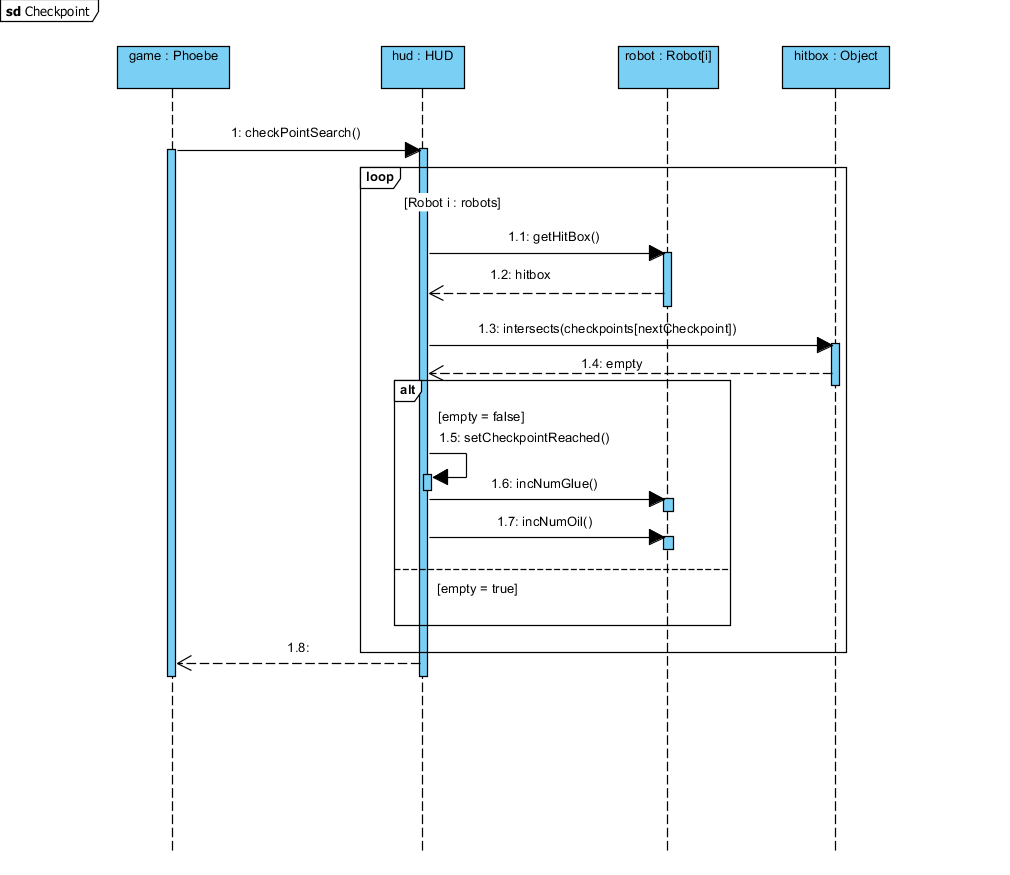
\includegraphics[width=17cm]{images/CheckpointSearch.PNG}
\caption{Következő checkpoint vizsgálata}
\label{fig:example2}
\end{center}
\end{figure}
\pagebreak

\subsection{Robot::CollisonWithObstacle}
\begin{figure}[h]
\begin{center}
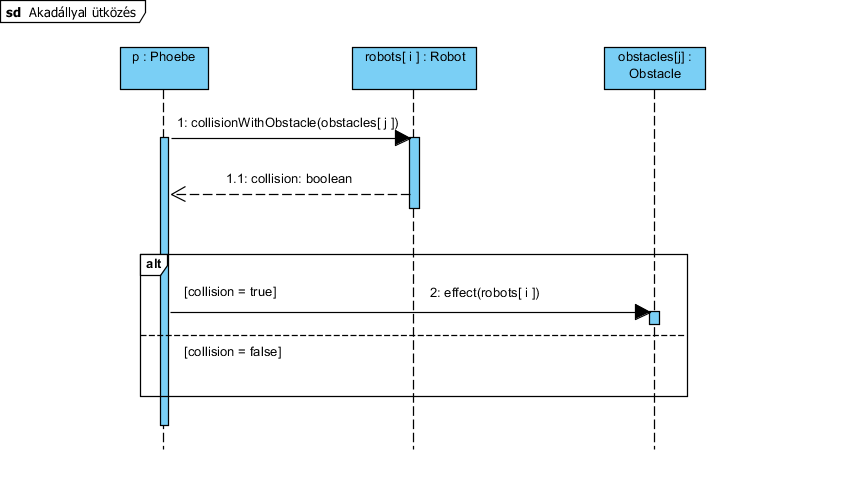
\includegraphics[width=17cm]{images/collisionWithObstacle()_sequence.PNG}
\caption{Robot ütközése akadállyal}
\label{fig:example4}
\end{center}
\end{figure}
\pagebreak

\subsection{Robot::CollisionWithRobot}
\begin{figure}[h]
\begin{center}
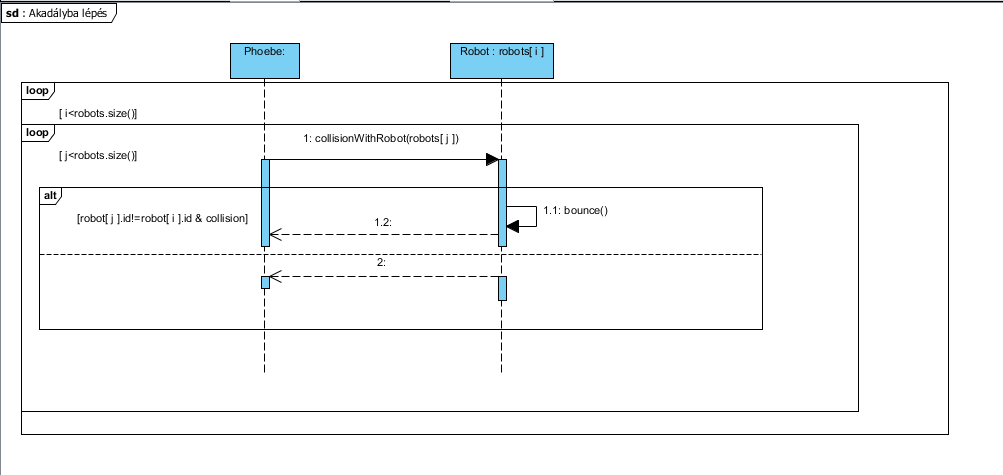
\includegraphics[width=17cm]{images/collisionWithRobot()_sequence.PNG}
\caption{Robot ütközése másik robottal}
\label{fig:example5}
\end{center}
\end{figure}
\pagebreak

\subsection{Robot::FallDown}
\begin{figure}[h]
\begin{center}
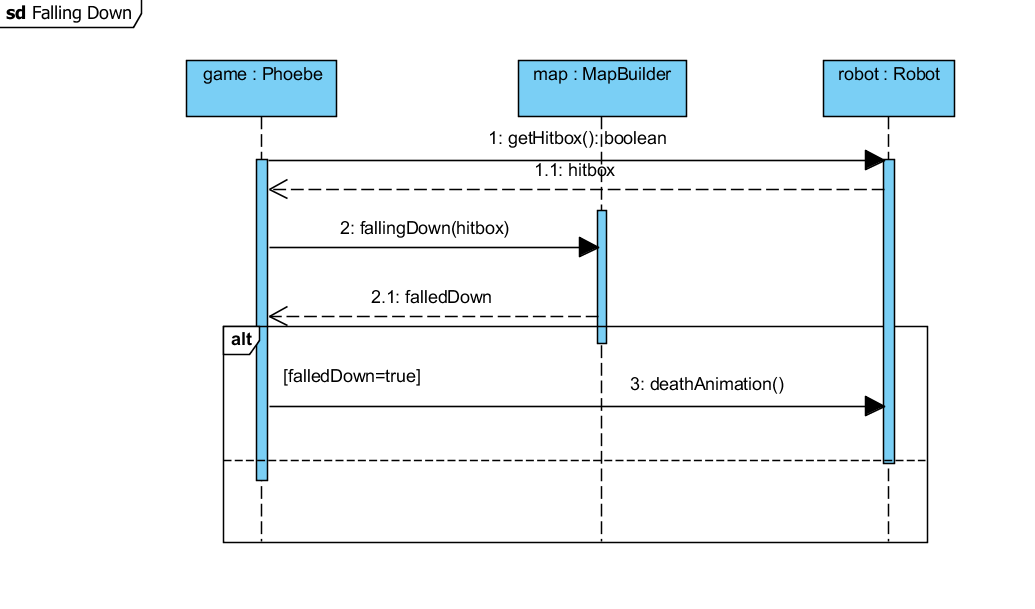
\includegraphics[width=17cm]{images/FallingDown.PNG}
\caption{Robot leesése a pályáról}
\label{fig:example6}
\end{center}
\end{figure}
\pagebreak

\subsection{Robot::InitGame}
\begin{figure}[h]
\begin{center}
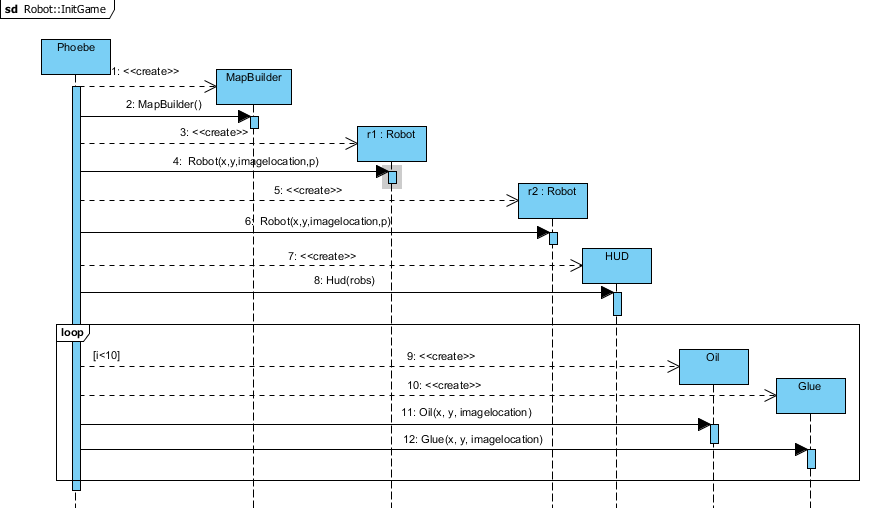
\includegraphics[width=17cm]{images/RobotInitGame.PNG}
\caption{A játék inicializálása}
\label{fig:example7}
\end{center}
\end{figure}
\pagebreak

\subsection{Robot::Move}
\begin{figure}[h]
\begin{center}
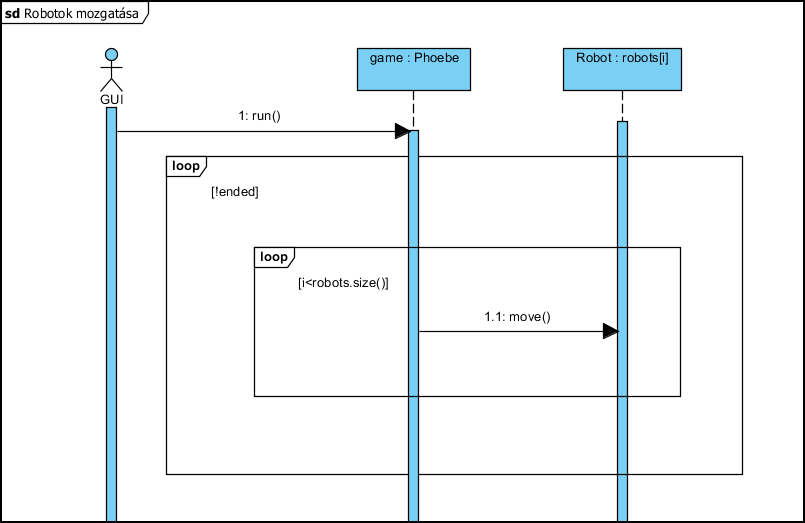
\includegraphics[width=17cm]{images/RobotMove.png}
\caption{A robot mozgatása}
\label{fig:example8}
\end{center}
\end{figure}
\pagebreak

\subsection{Robot::NewObstacle}
\begin{figure}[h]
\begin{center}
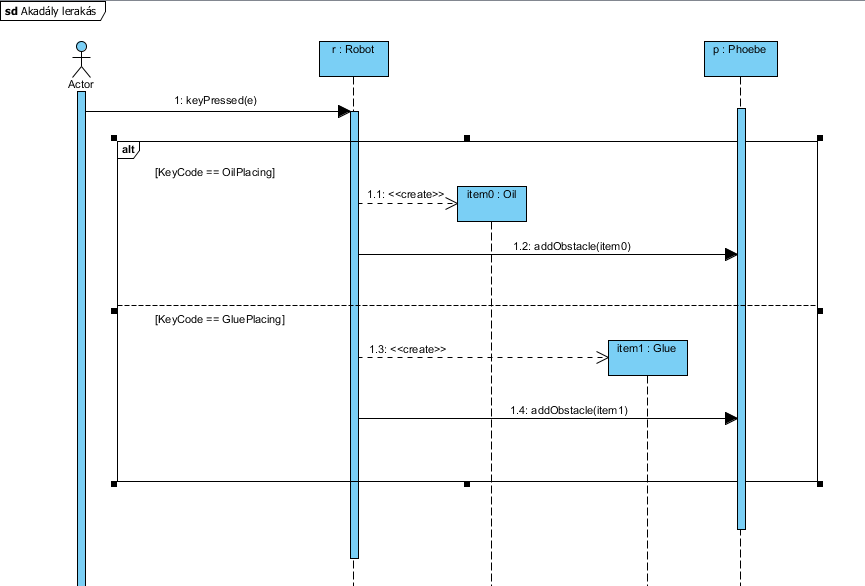
\includegraphics[width=17cm]{images/RobotAddObstacle.png}
\caption{Akadály lerakása}
\label{fig:example9}
\end{center}
\end{figure}
\pagebreak

\subsection{Robot::Settings}
\begin{figure}[h]
\begin{center}
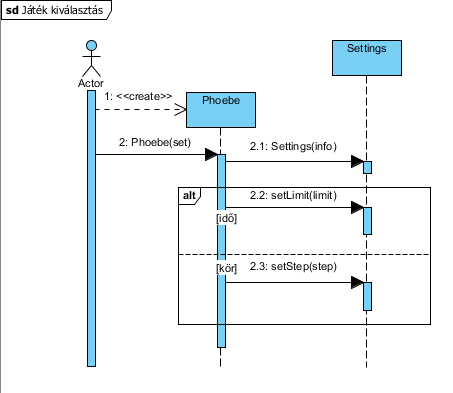
\includegraphics[width=17cm]{images/kivalasztas.PNG}
\caption{A játék beállításainak kiválasztása}
\label{fig:example10}
\end{center}
\end{figure}
\pagebreak

\subsection{Robot::End}
\begin{figure}[h]
\begin{center}
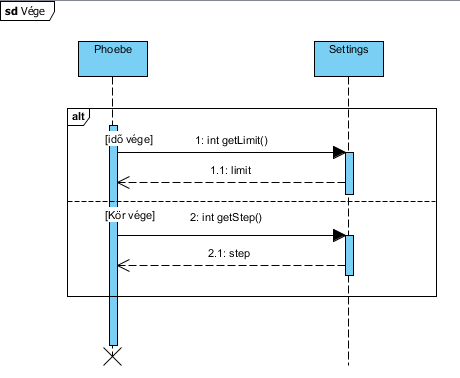
\includegraphics[width=17cm]{images/end.PNG}
\caption{Játék vége}
\label{fig:example11}
\end{center}
\end{figure}
\pagebreak

\section{Kommunikációs diagramok}

\subsection{Robot::CheckpointSearch}
\begin{figure}[h]
\begin{center}
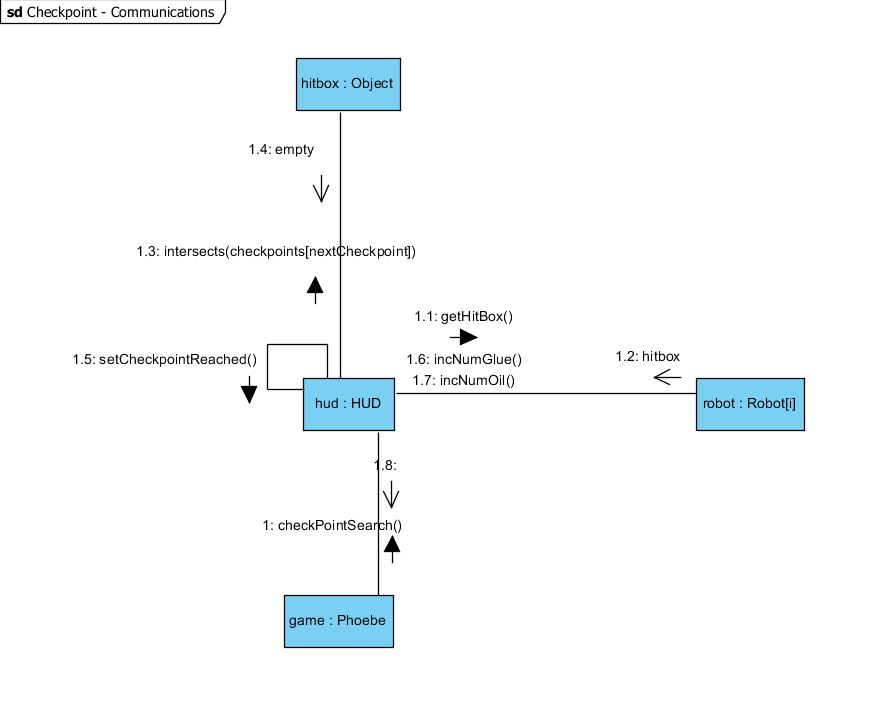
\includegraphics[width=17cm]{images/Commdiagrams/Comm_CheckpointSearch.jpg}
\caption{Következő checkpoint vizsgálata}
\label{fig:example2}
\end{center}
\end{figure}
\pagebreak

\subsection{Robot::CollisonWithObstacle}
\begin{figure}[h]
\begin{center}
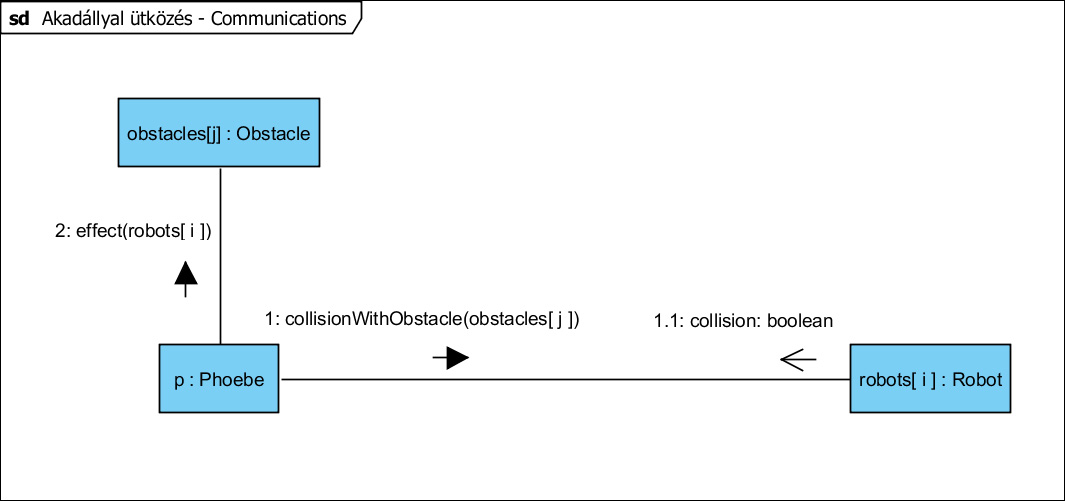
\includegraphics[width=17cm]{images/Commdiagrams/Comm_CollisionWithObstacle.jpg}
\caption{Robot ütközése akadállyal}
\label{fig:example4}
\end{center}
\end{figure}
\pagebreak

\subsection{Robot::CollisionWithRobot}
\begin{figure}[h]
\begin{center}
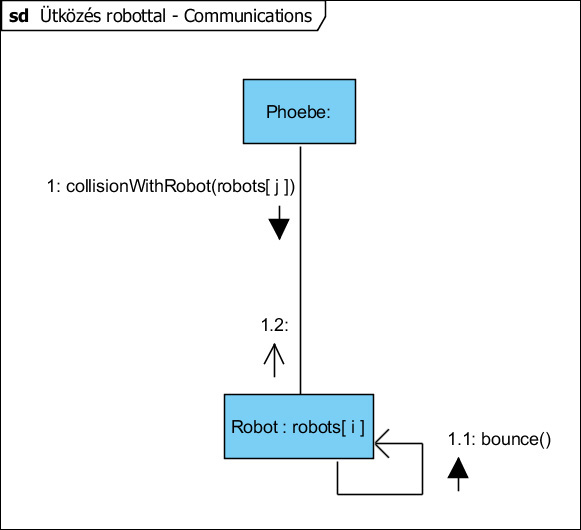
\includegraphics[width=17cm]{images/Commdiagrams/Comm_CollisionWithRobot.jpg}
\caption{Robot ütközése másik robottal}
\label{fig:example5}
\end{center}
\end{figure}
\pagebreak

\subsection{Robot::FallDown}
\begin{figure}[h]
\begin{center}
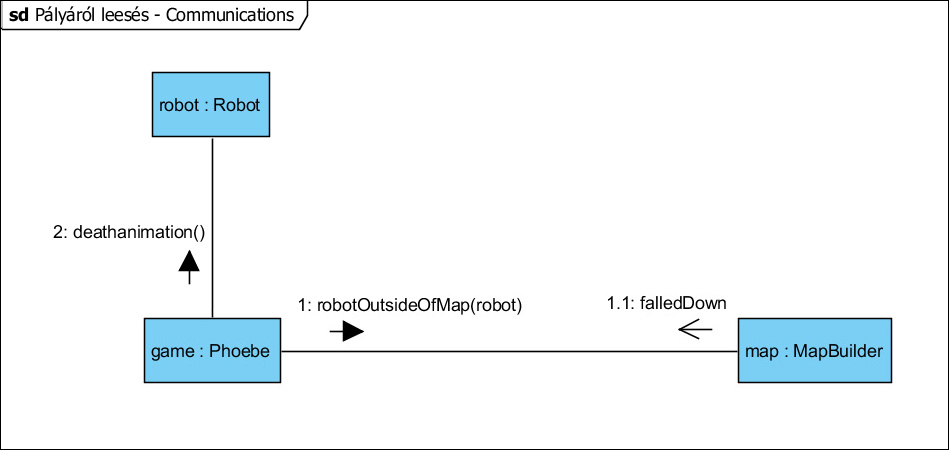
\includegraphics[width=17cm]{images/Commdiagrams/Comm_FallingDown.jpg}
\caption{Robot leesése a pályáról}
\label{fig:example6}
\end{center}
\end{figure}
\pagebreak

\subsection{Robot::InitGame}
\begin{figure}[h]
\begin{center}
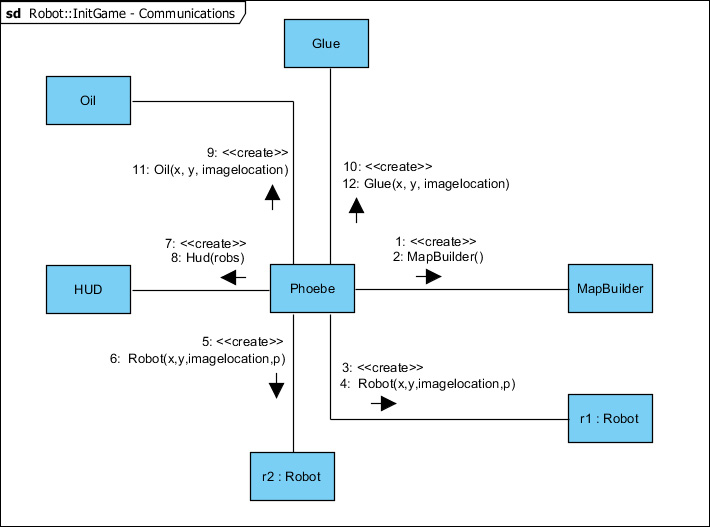
\includegraphics[width=17cm]{images/Commdiagrams/Comm_InitGame.jpg}
\caption{A játék inicializálása}
\label{fig:example7}
\end{center}
\end{figure}
\pagebreak

\subsection{Robot::Move}
\begin{figure}[h]
\begin{center}
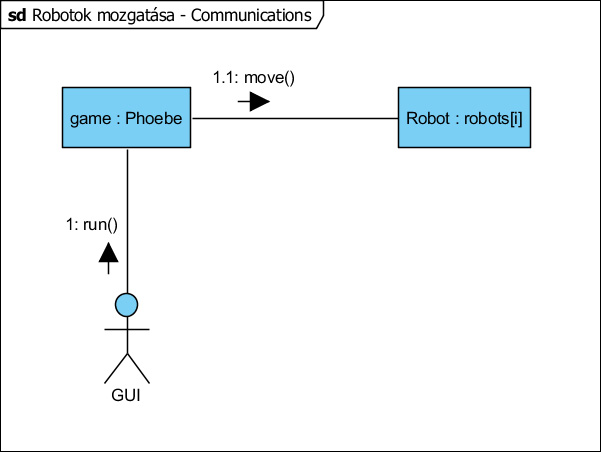
\includegraphics[width=17cm]{images/Commdiagrams/Comm_RobotMove.jpg}
\caption{A robot mozgatása}
\label{fig:example8}
\end{center}
\end{figure}
\pagebreak

\subsection{Robot::NewObstacle}
\begin{figure}[h]
\begin{center}
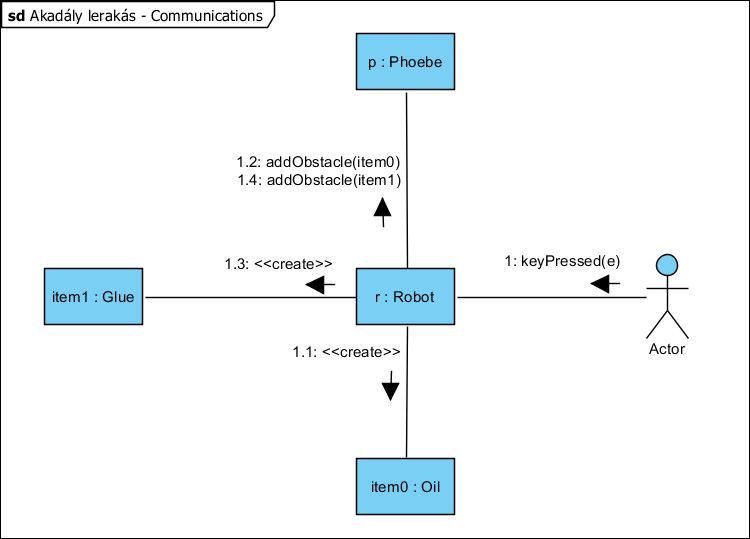
\includegraphics[width=17cm]{images/Commdiagrams/Comm_RobotAddObstacle.jpg}
\caption{Akadály lerakása}
\label{fig:example9}
\end{center}
\end{figure}
\pagebreak

\subsection{Robot::Settings}
\begin{figure}[h]
\begin{center}
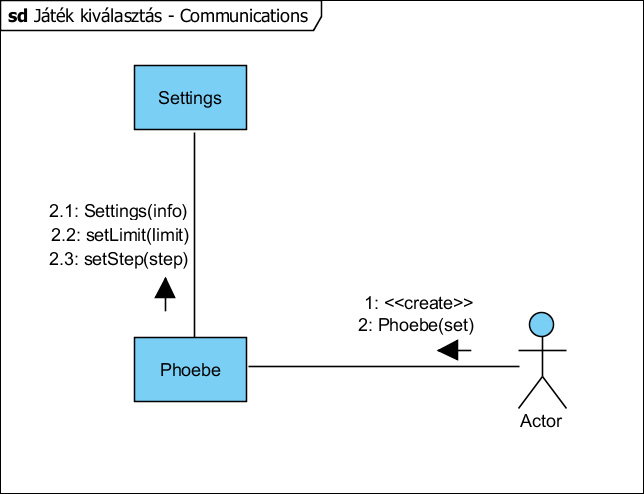
\includegraphics[width=17cm]{images/Commdiagrams/Comm_Settings.jpg}
\caption{A játék beállításainak kiválasztása}
\label{fig:example10}
\end{center}
\end{figure}
\pagebreak

\subsection{Robot::End}
\begin{figure}[h]
\begin{center}
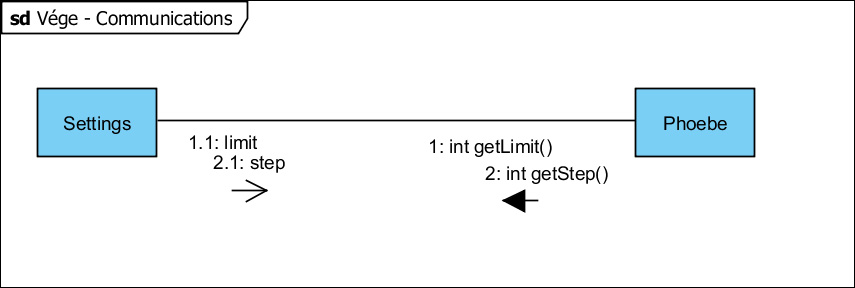
\includegraphics[width=17cm]{images/Commdiagrams/Comm_End.jpg}
\caption{Játék vége}
\label{fig:example11}
\end{center}
\end{figure}
\pagebreak